\documentclass[paper.tex]{subfiles}

\begin{document}




\section{Outline of proof that $\mathcal{V}$ is a universal template}

\begin{figure}[h]
  % not sure where to put this, but not here
  \centering
  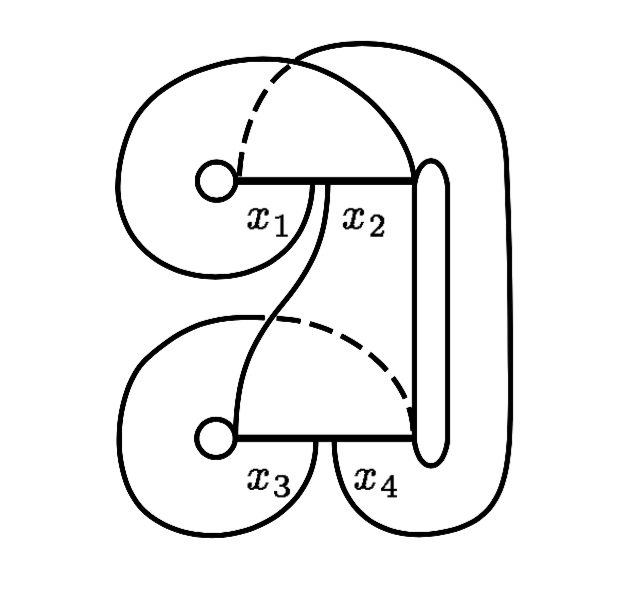
\includegraphics[width=0.5\textwidth]{universal}
  \caption{The universal template, reproduced from~\cite{knottyode}}\label{fig:universal}
\end{figure}

\subsection{Braids and the theorem of Alexander}

Every link is isotopic to some closed braid on $P$ strands for some $P$. Cite the proper paper

\subsection{The templates $\W_q$}

An isotopic copy of any closed braid exists as a set of periodic oribts on some $W_q$ for sufficently large $q$.

\subsection{Construct $\W_{q+1}$ from $\W_q$}

Start with renormalized $\W_1 \in \V$, and append a pair of ears to\dots

\subsection{Find $\W_q \subset \V$ for all $q$}

This is very tricky and will have to be very loosely sketched

This paper is referenced to prove this fact. (requires defining subtemplates; maybe that could be done in an earlier section)
https://www.math.upenn.edu/~ghrist/preprints/eraams.pdf

\end{document}
